\documentclass{article}
\usepackage{graphicx}
\usepackage{enumitem}
\usepackage{amsmath}
\usepackage{amsthm}
\usepackage{hyperref}
\newtheorem{theorem}{Theorem}
\newtheorem*{theorem1a}{Theorem 1-A}
\newtheorem*{corollary}{Corollary}
\newcommand{\manf}[1]{\mathbf{\mathcal{#1}}}
\newcommand{\vect}[1]{\mathbf{#1}}
\begin{document}
\title{A New Approach to Linear Filtering and Prediction Problems}
\author{R. E. KALMAN}
\date{}
\maketitle
\abstract{The classical filtering and prediction problem is re-examined using the Bode-Shannon representation of random processes and the “state transition” method of analysis of dynamic systems. New results are:
\begin{itemize}
\item[(1)] The formulation and methods of solution of the problem apply without modification to stationary and nonstationary statistics and to growing-memory and infinite-memory filters.
\item[(2)] A nonlinear difference (or differential) equation is derived for the covariance matrix of the optimal estimation error. From the solution of this equation the co-efficients of the difference (or differential) equation of the optimal linear filter are ob-tained without further calculations.
\item[(3)] The filtering problem is shown to be the dual of the noise-free regulator problem.
\end{itemize}

The new method developed here is applied to two well-known problems, confirming and extending earlier results.

The discussion is largely self-contained and proceeds from first principles; basic concepts of the theory of random processes are reviewed in the Appendix.}
\section{Introduction}
An important class of theoretical and practical problems in communication and control is of a statistical nature. Such problems are: (i) Prediction of random signals; (ii) separation of random signals from random noise; (iii) detection of signals of known form (pulses, sinusoids) in the presence of random noise.

In his pioneering work, Wiener [1] showed that problems (i) and (ii) lead to the so-called Wiener-Hopf integral equation; he also gave a method (spectral factorization) for the solution of this integral equation in the practically important special case of stationary statistics and rational spectra.

Many extensions and generalizations followed Wiener’s basic work. Zadeh and Ragazzini solved the finite-memory case [2]. Concurrently and independently of Bode and Shannon [3], they also gave a simplified method [2] of solution. Booton discussed the nonstationary Wiener-Hopf equation [4]. These results are now in standard texts [5-6]. A somewhat different approach along these main lines has been given recently by Darlington [7]. For extensions to sampled signals, see, e.g., Franklin [8], Lees [9]. Another approach based on the eigenfunctions of the Wiener-Hopf equation (which applies also to nonstationary problems whereas the preceding methods in general don’t), has been pioneered by Davis [10] and applied by many others, e.g., Shinbrot [11], Blum [12], Pugachev [13], Solodovnikov [14].

In all these works, the objective is to obtain the specification of a linear dynamic system (Wiener filter) which accomplishes the prediction, separation, or detection of a random signal.

Present methods for solving the Wiener problem are subject to a number of limitations which seriously curtail their practical usefulness:
\begin{itemize}
\item[(1)] The optimal filter is specified by its impulse response. It is not a simple task to synthesize the filter from such data.
\item[(2)] Numerical determination of the optimal impulse response is often quite involved and poorly suited to machine computation. The situation gets rapidly worse with increasing complexity of the problem.
\item[(3)] Important generalizations (e.g., growing-memory filters, nonstationary prediction) require new derivations, frequently of considerable difficulty to the nonspecialist.
\item[(4)] The mathematics of the derivations are not transparent. Fundamental assumptions and their consequences tend to be obscured.
\end{itemize}

This paper introduces a new look at this whole assemblage of problems, sidestepping the difficulties just mentioned. The following are the highlights of the paper:
\begin{itemize}
\item[(5)] \emph{Optimal Estimates and Orthogonal Projections}. The Wiener problem is approached from the point of view of conditional distributions and expectations. In this way, basic facts of the Wiener theory are quickly obtained; the scope of the results and the fundamental assumptions appear clearly. It is seen that all statistical calculations and results are based on first and second order averages; no other statistical data are needed. Thus difficulty (4) is eliminated. This method is well known in probability theory (see pp. 75--78 and 148--155 of Doob [15] and pp. 455--464 of Lo\`eve [16]) but has not yet been used extensively in engineering.
\item[(6)] \emph{Models for Random Processes}. Following, in particular, Bode and Shannon [3], arbitrary random signals are represented (up to second order average statistical properties) as the output of a linear dynamic system excited by independent or uncorrelated random signals (“white noise”). This is a standard trick in the engineering applications of the Wiener theory [2--7]. The approach taken here differs from the conventional one only in the way in which linear dynamic systems are described. We shall emphasize the concepts of state and state transition; in other words, linear systems will be specified by systems of first-order difference (or differential) equations. This point of view is natural and also necessary in order to take advantage of the simplifications mentioned under (5).
\item[(7)] \emph{Solution of the Wiener Problem}. With the state-transition method, a single derivation covers a large variety of problems: growing and infinite memory filters, stationary and nonstationary statistics, etc.; difficulty (3) disappears. Having guessed the “state” of the estimation (i.e., filtering or prediction) problem correctly, one is led to a nonlinear difference (or differential) equation for the covariance matrix of the optimal estimation error. This is vaguely analogous to the Wiener-Hopf equation. Solution of the equation for the covariance matrix starts at the time $t_0$ when the first observation is taken; at each later time $t$ the solution of the equation represents the covariance of the optimal prediction error given observations in the interval $(t_0, t)$. From the covariance matrix at time $t$ we obtain at once, without further calculations, the coefficients (in general, time-varying) characterizing the optimal linear filter.
\item[(8)] \emph{The Dual Problem}. The new formulation of the Wiener problem brings it into contact with the growing new theory of control systems based on the “state” point of view [17--24]. It turns out, \emph{surprisingly}, that the Wiener problem is the dual of the noise-free optimal regulator problem, which has been solved previously by the author, using the state-transition method to great advantage [18, 23, 24]. The mathematical background of the two problems is identical--this has been suspected all along, but until now the analogies have never been made explicit.
\item[(9)] \emph{Applications}. The power of the new method is most apparent in theoretical investigations and in numerical answers to complex practical problems. In the latter case, it is best to resort to machine computation. Examples of this type will be discussed later. To provide some feel for applications, two standard examples from nonstationary prediction are included; in these cases the solution of the nonlinear difference equation mentioned under (7) above can be obtained even in closed form.
\end{itemize}

For easy reference, the main results are displayed in the form of theorems. Only Theorems 3 and 4 are original. The next section and the Appendix serve mainly to review well-known material in a form suitable for the present purposes.

\section{Notation Coventions}
Throughout the paper, we shall deal mainly with \emph{discrete} (or \emph{sampled}) dynamic systems; in other words, signals will be observed at equally spaced points in time (\emph{sampling instants}). By suitable choice of the time scale, the constant intervals between successive sampling instants (\emph{sampling periods}) may be chosen as unity. Thus variables referring to time, such as $t$, $t_0$, $\tau$, $T$ will always be integers. The restriction to discrete dynamic systems is not at all essential (at least from the engineering point of view); by using the discreteness, however, we can keep the mathematics rigorous and yet elementary. Vectors will be denoted by small bold-face letters: $\mathbf{a}$, $\mathbf{b}$, $\dotsc$, $\mathbf{u}$, $\mathbf{x}$, $\mathbf{y}$, $\dotsc$ A vector or more precisely an $n$-vector is a set of $n$ numbers $x_1$, $\dotsc$ $x_n$; the $x_i$ are the \emph{co-ordinates} or components of the vector $\mathbf{x}$.

Matrices will be denoted by capital bold-face letters: $\mathbf{A}$, $\mathbf{B}$, $\mathbf{Q}$, $\boldsymbol{\Phi}$, $\boldsymbol{\Psi}$, $\dotsc$; they are $m \times n$ arrays of elements $a_{ij}$, $b_{ij}$, $q_{ij}$, $\dotsc$ The \emph{transpose} (interchanging rows and columns) of a matrix will be denoted by the prime. In manipulating formulas, it will be convenient to regard a vector as a matrix with a single column.

Using the conventional definition of matrix multiplication, we write the \emph{scalar product} of two $n$-vector $\mathbf{x}$, $\mathbf{y}$ as
\begin{equation*}
\mathbf{x'y}=\sum^n_{i=1}x_iy_i=\mathbf{y'x}
\end{equation*}
The scalar product is clearly a scalar, i.e., not a vector, quantity. Similarly, the quadratic form associated with the $n \times n$ matrix $\mathbf{Q}$ is,
\begin{equation*}
\mathbf{x'Qx}=\sum^n_{i,j=1}x_i q_{ij} x_j
\end{equation*}
We define the expression $\mathbf{xy'}$ where $\mathbf{x'}$ is an $m$-vector and $\mathbf{y}$ is an $n$-vector to be the $m \times n$ matrix with elements $x_i y_j$.

We write $E(\mathbf{x}) = E\mathbf{x}$ for the expected value of the random vector $\mathbf{x}$ (see Appendix). It is usually convenient to omit the brackets after $E$. This does not result in confusion in simple cases since constants and the operator $E$ commute. Thus $E\mathbf{xy'} =$ matrix with elements $E(x_i y_j)$; $E\mathbf{x}E\mathbf{y'} =$ matrix with elements $E(x_i)E(y_j)$.

For ease of reference, a list of the principal symbols used is given below.
\begin{table}[htbp]
\centering
\begin{tabular}{rl}
\multicolumn{2}{l}{\textbf{Optimal Estimates}}\\
$t$ & time in general, present time.\\
$t_0$ & time at which observations start.\\
$x_1(t),x_2(t)$ & basic random variables.\\
$y(t)$ & observed random variable.\\
$x^\ast (t_1 \vert t)$ & optimal estimate of $x_1(t_1)$ given $y(t_0), \dotsc, y(t)$\\
$L$ & loss function (non random function of its argument).\\
$\epsilon$ & estimation error (random variable).\\
\multicolumn{2}{l}{\textbf{Orthogonal Projections}}\\
$\mathbf{\mathcal{Y}}(t)$ & linear manifold generated by the random variables $y(t_0), \dotsc, y(t)$.\\
$\bar{x}(t_1 \vert t)$ & orthogonal projection of $x(t_1)$ on $\mathbf{\mathcal{Y}}(t)$.\\
$\tilde{x}(t_1 \vert t)$ & component of $x(t_1)$ orthogonal to $\mathbf{\mathcal{Y}}(t)$.\\
\multicolumn{2}{l}{\textbf{Models for Random Processes}}\\
$\boldsymbol{\Phi}(t+1 ; t)$ & transition matrix\\
$\mathbf{Q}(t)$ & covariance of random excitation\\
\multicolumn{2}{l}{\textbf{Solution of the Wiener Problem}}\\
$\mathbf{x}(t)$ & basic random variable.\\
$\mathbf{y}(t)$ & observed random variable.\\
$\manf{Y}(t)$ & linear manifold generated by $\mathbf{y}(t_0), \dotsc, \mathbf{y}(t)$.\\
$\manf{Z}(t)$ & linear manifold generated by $\tilde{\mathbf{y}}(t \vert t-1)$.\\
$\mathbf{x}^\ast(t_1 \vert t)$ & optimal estimate of $\mathbf{x}(t_1)$ given $\manf{Y}(t)$.\\
$\tilde{\mathbf{x}}(t_1 \vert t)$ & error in optimal estimate of $\mathbf{x}(t_1)$ given $\manf{Y}(t)$.
\end{tabular}
\end{table}

\section{Optimal Estimates}
To have a concrete description or the type of problems to be studied, consider the following situation. We are given signal $x_1(t)$ and noise $x_2(t)$. Only the sum $y(t) = x_1(t) + x_2(t)$ can be observed. Suppose we have observed and know exactly the values of $y(t0)$, $\dotsc$, $y(t)$. What can we infer from this knowledge in regard to the (unobservable) value of the signal at $t = t_1$, where $t_1$ may be less than, equal to, or greater than $t$? If $t_1 < t$, this is a \emph{data-smoothing (interpolation)} problem. If $t_1 = t$, this is called \emph{filtering}. If $t_1 > t$, we have a \emph{prediction} problem. Since our treatment will be general enough to include these and similar problems, we shall use hereafter the collective term \emph{estimalion}.

As was pointed out by Wiener [1], the natural setting of the estimation problem belongs to the realm of probability theory and statistics. Thus signal, noise, and their sum will be random variables, and consequently they may be regarded as random processes. From the probabilistic description of the random processes we can determine the probability with which a particular sample of the signal and noise will occur. For any given set of measured values $\eta(t_0)$, $\dotsc$, $\eta(t)$ of the random variable $y(t)$ one can then also determine, in principle, the probability of simultaneous occurrence of various values $\xi_1(t)$ of the random variable $x_1(t_1)$. This is the conditional probability distribution function
\begin{equation}
\label{eq1}
Pr[x_1(t_1) \le \xi_1 \vert y(t_0)=\eta(t_0), \dotsc, y(t)=\eta(t)]=F(\xi_1)
\end{equation}

Evidently, $F(\xi_1)$ represents all the information which the measurement of the random variables $y(t_0)$, $\dotsc$, $y(t)$ has conveyed about the random variable $x_1(t_1)$. Any statistical estimate of the random variable $x_1(t_1)$ will be some function of this distribution and therefore a (nonrandom) function of the random variables $y(t_0)$, $\dotsc$, $y(t)$. This statistical estimate is denoted by $X_1(t_1 \vert t)$, or by just $X_1(t_1)$ or $X_1$ when the set of observed random variables or the time at which the estimate is required are clear from context.

Suppose now that X1 is given as a fixed function of the random variables $y(t_0)$, $\dotsc$, $y(t)$. Then $X_1$ is itself a random variable and its actual value is known whenever the actual values of $y(t_0)$, $\dotsc$, $y(t)$ are known. In general, the actual value of $X_1(t_1)$ will be different from the (unknown) actual value of $x_1(t_1)$. To arrive at a rational way of determining $X_1$, it is natural to assign a penalty or loss for incorrect estimates. Clearly, the loss should be a (i) positive, (ii) nondecreasing function of the estimation error $\epsilon = x_1(t_1)-X_1(t_1)$. Thus we define a \emph{loss function} by
\begin{equation*}
L(0)=0
\end{equation*}
\begin{equation}
\label{eq2}
L(\epsilon_2) \le L(\epsilon_1) \le 0 \text{ when } \epsilon_2 \le \epsilon_1 \le 0
\end{equation}
\begin{equation*}
L(\epsilon)=L(-\epsilon) 
\end{equation*}
Some common examples of loss functions are: $L(\epsilon) = a\epsilon^2$, $a\epsilon^4$, $a\vert \epsilon \vert$, $a[1 - \exp(-\epsilon^2)]$, etc., where $a$ is a positive constant.

One (but by no means the only) natural way of choosing the random variable $X_1$ is to require that this choice should minimize the average loss or risk
\begin{equation}
\label{eq3}
E\{L[x_1(t_1)-X_1(t_1)]\}=E[E\{L[x(t_1)-X_1(t_1)] \vert y(t_0), \dotsc, y(t)\}]
\end{equation}
Since the first expectation on the right-hand side of (\ref{eq3}) does not depend on the choice of $X_1$ but only on $y(t_0)$, $\dotsc$, $y(t)$, it is clear that minimizing (\ref{eq3}) is equivalent to minimizing
\begin{equation}
\label{eq4}
E\{L[x_1(t_1)-X_1(t_1)] \vert y(t_0), \dotsc, y(t)\}
\end{equation}
Under just slight additional assumptions, optimal estimates can be characterized in a simple way.

\begin{theorem}
\label{th1}
Assume that L is of type (\ref{eq2}) and that the conditional distribution function $F(\xi)$ defined by (\ref{eq1}) is:
\begin{itemize}
\item[A] symmetric about the mean $\bar{\xi}$:
    \begin{equation*}
    F(\xi-\bar{\xi})=1-F(\bar{\xi}-xi)
    \end{equation*}
\item[B] convex for $\xi \le \bar{\xi}$:
    \begin{multline*}
    F(\lambda\xi_1+(1-\lambda)\xi_2) \le \lambda F(\xi_1)+(1-\lambda)F(\xi_2)\\
    \text{for all }\xi_1,\xi_2 \le \bar{\xi} \text{ and } 0 \le \lambda \le 1
    \end{multline*}
for all $\xi_1$, $\xi_2 \le \xi$ and $0 \le \lambda \le 1$
\end{itemize}
Then the random variable $x_1^\ast(t_1 \vert t)$ which minimizes the average loss (\ref{eq3}) is the conditional expectation
\begin{equation}
\label{eq5}
x^{\ast}_1(t_1 \vert t)=E[x_1(t_1) \vert y(t_0),\dotsc,y(t)]
\end{equation}
\end{theorem}

\textbf{Proof:} As pointed out recently by Sherman [25], this theorem follows immediately from a well-known lemma in probability theory.
\begin{corollary}
If the random processes $\{x_1(t)\}$, $\{x_2(t)\}$, and $\{y(t)\}$ are gaussian, Theorem \ref{th1} holds.
\end{corollary}
\textbf{Proof:} By Theorem 5, (A) (see Appendix), conditional distributions on a gaussian random process are gaussian. Hence the requirements of Theorem \ref{th1} are always satisfied.

In the control system literature, this theorem appears sometimes in a form which is more restrictive in one way and more general in another way:
\begin{theorem1a}
\label{th1a}
If $L(\epsilon) = \epsilon^2$, then Theorem \ref{th1} is true without assumptions (A) and (B).
\end{theorem1a}

\textbf{Proof:} Expand the conditional expectation (\ref{eq4}):
\begin{equation*}
E[x_1^2(t_1) \vert y(t_0),\dotsc,y(t)]-2X_1(t_1)E[x_1(t_1) \vert y(t_0),\dotsc,y(t)]+X_1^2(t_1)
\end{equation*}
and differentiate with respect to $X_1(t_1)$. This is not a completely rigorous argument; for a simple rigorous proof see Doob [15], pp. 77-78.

\textbf{Remarks.}(a) As far as the author is aware, it is not known what is the most general class of random processes ${x_1(t)}$, ${x_2(t)}$ for which the conditional distribution function satisfies the requirements of Theorem \ref{th1}.

(b) Aside from the note of Sherman, Theorem \ref{th1} apparently has never been stated explicitly in the control systems literature. In fact, one finds many statements to the effect that loss functions of the general type (\ref{eq2}) cannot be conveniently handled mathematically.

(c) In the sequel, we shall be dealing mainly with vectorvalued random variables. In that case, the estimation problem is stated as: Given a vector-valued random process ${\mathbf{x}(t)}$ and observed random variables $\mathbf{y}(t_0)$, $\dotsc$, $\mathbf{y}(t)$, where $\mathbf{y}(t) = \mathbf{M}\mathbf{x}(t)$ ($\mathbf{M}$ being a singular matrix; in other words, not all co-ordinates of $\mathbf{x}(t)$ can be observed), find an estimate $\mathbf{X}(t_1)$ which minimizes the expected loss $E[L(\Vert x(t_1) - X(t_1)\Vert)]$, $\Vert$ $\Vert$ being the norm of a vector. Theorem \ref{th1} remains true in the vector case also, provided we require that the conditional distribution function of the n coordinates of the vector $\mathbf{x}(t_1)$,
\begin{equation*}
Pr[x_1(t_1) \le \xi_1,\dotsc,x_n(t_1) \le \xi_n \vert \mathbf{y}(t_0),\dotsc,\mathbf{y}(t)]=F(\xi_1,\dotsc,\xi_n)
\end{equation*}
be symmetric with respect to the n variables $\xi_1 - \bar{xi}_1$, $\dotsc$, $\xi_n - \bar{\xi}_n$ and convex in the region where all of these variables are negative.

\section{Orthogonal Projections}
The explicit calculation of the optimal estimate as a function of the observed variables is, in general, impossible. There is an important exception: The processes $\{x_1(t)\}$, $\{x_2(t)\}$ are gaussian.

On the other hand, if we attempt to get an optimal estimate under the restriction $L(\epsilon) = \epsilon^2$ and the additional requirement that the estimate be a linear function of the observed random variables, we get an estimate which is identical with the optimal estimate in the gaussian case, without the assumption of linearity or quadratic loss function. This shows that results obtainable by linear estimation can be bettered by nonlinear estimation only when (i) the random processes are nongaussian and even then (in view of Theorem 5, (C)) only (ii) by considering at least thirdorder probability distribution functions.

In the special cases just mentioned, the explicit solution of the estimation problem is most easily understood with the help of a geometric picture. This is the subject of the present section.

Consider the (real-valued) random variables $y(t_0)$, $\dotsc$, $y(t)$. The set of all linear combinations of these random variables with real
coefficients
\begin{equation}
\label{eq6}
\sum^t_{i=t_0}a_i y(i)
\end{equation}
forms a \emph{vector space (linear manifold)} which we denote by $\mathbf{\mathcal{Y}}(t)$. We regard, abstractly, any expression of the form (\ref{eq6}) as “point” or “vector” in $\manf{Y}(t)$; this use of the word “vector” should not be confused, of course, with “vector-valued” random variables, etc. Since we do not want to fix the value of $t$ (i.e., the total number of possible observations), $\manf{Y}(t)$ should be regarded as a finitedimensional subspace of the space of all possible observations.

Given any two vectors $u$, $v$ in $\manf{Y}(t)$ (i.e., random variables expressible in the form (\ref{eq6})), we say that $u$ and $v$ are \emph{orthogonal} if $Euv = 0$. Using the Schmidt orthogonalization procedure, as described for instance by Doob [15], p. 151, or by Lo\`{e}ve [16], p. 459, it is easy to select an \emph{orthonormal basis} in $\manf{Y}(t)$. By this is meant a set of vectors $e_{t_0}$, $\dotsc$, $e_t$ in $\manf{Y}(t)$ such that any vector in $\manf{Y}(t)$ can be expressed as a unique linear combination of $e_{t_0}$, $\dotsc$, $e_t$ and
\begin{equation}
\label{eq7}
\left.\begin{aligned}
Ee_ie_j=\delta_{ij}&=1 \text{ if } i = j\\
&=0 \text{ if } i \ne j
\end{aligned}\right\}
\qquad (i,j=t_0,\dotsc,t)
\end{equation}
Thus any vector $\bar{x}$ in $\manf{Y}(t)$. is given by
\begin{equation*}
\bar{x}=\sum^t_{i=t_0}a_ie_i
\end{equation*}
and so the coefficients $a_i$ can be immediately determined with the
aid of (\ref{eq7}):
\begin{equation}
\label{eq8}
E\bar{x}e_j=E[\sum^t_{i=t_0}a_ie_i]e_j=\sum^t_{i=t_0}a_iEe_ie_j=\sum^t_{i=t_0}\delta_{ij}=a_j
\end{equation}

It follows further that any random variable $x$ (not necessarily in $\manf{Y}(t)$) can be uniquely decomposed into two parts: a part $\bar{x}$ in $\manf{Y}(t)$ and a part $\tilde{x}$ orthogonal to $\manf{Y}(t)$ (i.e., orthogonal to every vector in $\manf{Y}(t)$). In fact, we can write
\begin{equation}
\label{eq9}
x=\bar{x}+\tilde{x}=\sum^t_{i=t_0}(Exe_i)e_i+\tilde{x}
\end{equation}

Thus $\bar{x}$ is uniquely determined by equation (\ref{eq9}) and is obviously a vector in $\manf{Y}(t)$. Therefore $\tilde{x}$ is also uniquely determined; it remains to check that it is orthogonal to $\manf{Y}(t)$:
\begin{equation*}
E\tilde{x}e_i=E(x-\bar{x})e_i=Exe_i-E\bar{x}e_i
\end{equation*}

Now the co-ordinates of $\bar{x}$ with respect to the basis $e_{t_0}$, $\dotsc$, $e_t$, are given either in the form $E\bar{x}e_i$ (as in (\ref{eq8})) or in the form $Exe_i$ (as in (\ref{eq9})). Since the co-ordinates are unique, $Exe_i = E\bar{x}e_i$ ($i = t_0, ..., t$); hence $E\tilde{x}e_i = 0$ and $\tilde{x}$ is orthogonal to every base vector $e_i$; and therefore to $\manf{Y}(t)$. We call $\bar{x}$ the \emph{orthogonal projection} of $x$ on $\manf{Y}(t)$.

There is another way in which the orthogonal projection can be characterized: $\bar{x}$ is that vector in $\manf{Y}(t)$ (i.e., that linear function of the random variables $y(t_0)$, $\dotsc$, $y(t)$) which minimizes the quadratic loss function. In fact, if $\bar{w}$ is any other vector in $\manf{Y}(t)$, we have
\begin{equation*}
E(x-\bar{w})^2=E(\tilde{x}+\bar{x}-\bar{w})^2=E[(x-\bar{x})+(\bar{x}-\bar{w})]^2
\end{equation*}

Since $\tilde{x}$ is orthogonal to every vector in $\manf{Y}(t)$ and in particular to $\bar{x} - \bar{w}$ we have
\begin{equation}
\label{eq10}
E(x-\bar{w})^2=E(x-\bar{x})^2+E(\bar{x}-\bar{w})^2 \ge E(x-\bar{x})^2
\end{equation}
This shows that, if $\bar{w}$ also minimizes the quadratic loss, we must have $E(\bar{x} - \bar{w})^2 = 0$ which means that the random variables $\bar{x}$ and $\bar{w}$ are equal (except possibly for a set of events whose probability is zero).

These results may be summarized as follows:
\begin{theorem}
\label{th2}
Let $\{x(t)\}$, $\{y(t)\}$ random processes with zero mean (i.e., $Ex(t) = Ey(t) = 0$ for all $t$). We observe $y(t_0)$, $\dotsc$, $y(t)$.

If either
\begin{itemize}
\item[A] the random processes $\{x(t)\}$, $\{y(t)\}$ are gaussian; or
\item[B] the optimal estimate is restricted to be a linear function of the observed random variables and $L(\epsilon) = \epsilon^2$;
\end{itemize}
then
\begin{multline}
\label{eq11}
x^\ast (t_1 \vert t) = \text{optimal estimate of }x(t_1)\text{ given }y(t_0),\dotsc,y(t)\\
=\text{orthogonal projection }\bar{x}(t_1 \vert t)\text{ of }x(t_1)\text{ on }\mathbf{\mathcal{Y}}(t)。
\end{multline}
\end{theorem}

These results are well-known though not easily accessible in the control systems literature. See Doob [15], pp. 75–78, or Pugachev [26]. It is sometimes convenient to denote the orthogonal projection by
\begin{equation*}
\bar{x}(t_1 \vert t) \equiv x^\ast (t_1 \vert t)=\hat{E}[x(t_1) \vert \mathbf{\mathcal{Y}}(t)]
\end{equation*}

The notation $\hat{E}$ is motivated by part (b) of the theorem: If the stochastic processes in question are gaussian, then orthogonal projection is actually identical with conditional expectation. 

\textbf{Proof.} (A) This is a direct consequence of the remarks in connection
with (\ref{eq10}).

(B) Since $x(t)$, $y(t)$ are random variables with zero mean, it is clear from formula (\ref{eq9}) that the orthogonal part $\tilde{x}(t_1 \vert t)$ of $x(t_1)$ with respect to the linear manifold $\manf{Y}(t)$ is also a random variable with zero mean. Orthogonal random variables with zero mean are uncorrelated; if they are also gaussian then (by Theorem 5 (B)) they are independent. Thus
\begin{equation*}
\begin{split}
0=E\tilde{x}(t_1 \vert t)&=E[\tilde{x}(t_1 \vert t)\vert y(t_0),\dotsc,y(t)]\\
&=E[x(t_1) - \bar{x}(t_1 \vert t)\vert y(t_0),\dotsc,y(t)]\\
&=E[x(t_1)\vert y(t_0),\dotsc,y(t)]-\bar{x}(t_1 \vert t)=0
\end{split}
\end{equation*}

\textbf{Remarks.} (d) A rigorous formulation of the contents of this section as $t \to \infty$ requires some elementary notions from the theory of Hilbert space. See Doob [15] and Lo\`{e}ve [16].

(e) The physical interpretation of Theorem \ref{th2} is largely a matter of taste. If we are not worried about the assumption of gaussianness,
part (A) shows that the orthogonal projection is the optimal estimate for all reasonable loss functions. If we do worry about gaussianness, even if we are resigned to consider only linear estimates, we know that orthogonal projections are not the optimal estimate for many reasonable loss functions. Since in practice it is difficult to ascertain to what degree of approximation a random process of physical origin is gaussian, it is hard to decide whether Theorem \ref{th2} has very broad or very limited significance.

(f) Theorem \ref{th2} is immediately generalized for the case of vector-valued random variables. In fact, we define the linear manifold $\manf{Y}(t)$ generated by $y(t_0)$, $\dotsc$, $y(t)$ to be the set of all linear combinations
\begin{equation*}
\sum^t_{i=t_0}\sum^m_{j=1}a_{ij}y_j (i)
\end{equation*}
of all $m$ co-ordinates of each of the random vectors $y(t_0)$, $\dotsc$, $y(t)$. The rest of the story proceeds as before.
(g) Theorem \ref{th2} states in effect that the optimal estimate under conditions (A) or (B) is a linear combination of all previous observations. In other words, the optimal estimate can be regarded as the output of a linear filter, with the input being the actually occurring values of the observable random variables; Theorem \ref{th2} gives a way of computing the impulse response of the optimal filter. As pointed out before, knowledge of this impulse response is not a complete solution of the problem; for this reason, no explicit formulas for the calculation of the impulse response will be given.
\section{Models for Random Processes}
In dealing with physical phenomena, it is not sufficient to give
an empirical description but one must have also some idea of the
underlying causes. Without being able to separate in some sense
causes and effects, i.e., without the assumption of causality, one
can hardly hope for useful results.

It is a fairly generally accepted fact that primary macroscopic
sources of random phenomena are independent gaussian processes.
5 A well-known example is the noise voltage produced in a
resistor due to thermal agitation. In most cases, observed random
phenomena are not describable by independent random variables.
The statistical dependence (correlation) between random signals
observed at different times is usually explained by the presence of
a dynamic system between the primary random source and the
observer. Thus a random function of time may be thought of as the
output of a dynamic system excited by an independent gaussian
random process.

An important property of gaussian random signals is that they
remain gaussian after passing through a linear system (Theorem 5
(A)). Assuming independent gaussian primary random sources, if
the observed random signal is also gaussian, we may assume that
the dynamic system between the observer and the primary source
is linear. This conclusion may be forced on us also because of
lack of detailed knowledge of the statistical properties of the
observed random signal: Given any random process with known
first and second-order averages, we can find a gaussian random
process with the same properties (Theorem 5 (C)). Thus gaussian
distributions and linear dynamics are natural, mutually plausible
assumptions particularly when the statistical data are scant.

How is a dynamic system (linear or nonlinear) described? The
fundamental concept is the notion of the state. By this is meant,
intuitively, some quantitative information (a set of numbers, a
function, etc.) which is the least amount of data one has to know
about the past behavior of the system in order to predict its future
behavior. The dynamics is then described in terms of state
transitions, i.e., one must specify how one state is transformed
into another as time passes.

A linear dynamic system may be described in general by the
vector differential equation
\begin{equation}
\label{eq12}
\left.\begin{aligned}
&d\mathbf{x}/dt=\mathbf{F}(t)\mathbf{x}+\mathbf{D}(t)\mathbf{u}(t)\\
\text{ and }\qquad&\\
&\mathbf{y}(t)=\mathbf{M}(t)\mathbf{x}(t)
\end{aligned}\right\}
\end{equation}
where x is an n-vector, the state of the system (the components xi
of x are called state variables); u(t) is an m-vector (m ≤ n)
representing the inputs to the system; F(t) and D(t) are n × n,
respectively, n × m matrices. If all coefficients of F(t), D(t), M(t)
are constants, we say that the dynamic system (12) is timeinvariant
or stationary. Finally, y(t) is a p-vector denoting the
outputs of the system; M(t) is an n × p matrix; p ≤ n

\begin{figure}[htbp]
\centering
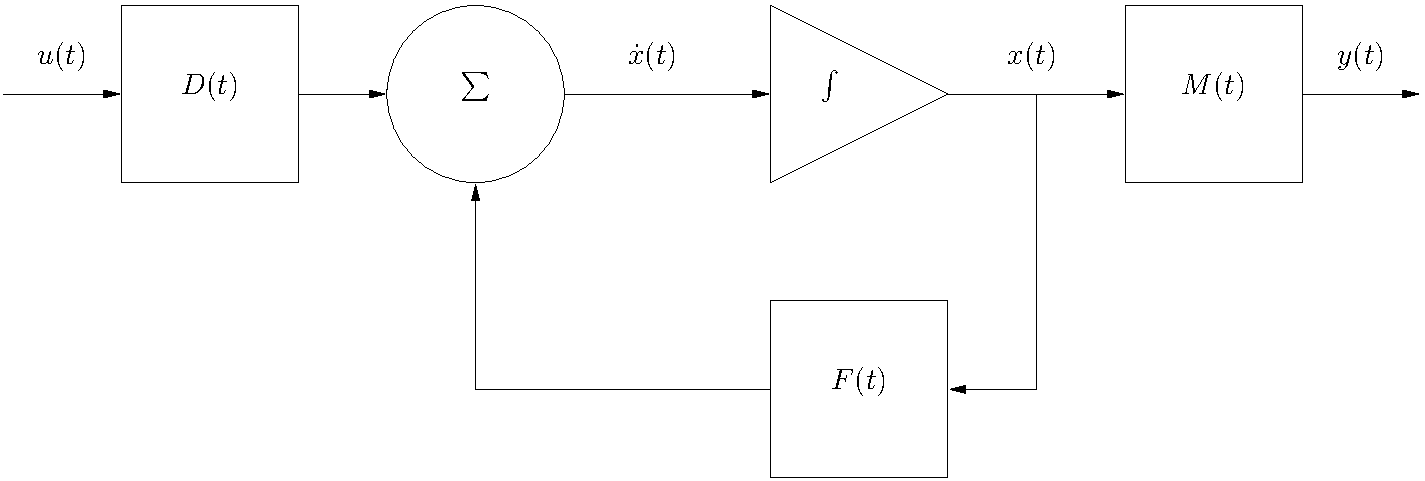
\includegraphics[width=0.5\paperwidth]{fig/fg1.pdf}
\caption{Matrix block diagram of the general linear continuous-dynamic system}
\label{fg1}
\end{figure}

The physical interpretation of (12) has been discussed in detail
elsewhere [18, 20, 23]. A look at the block diagram in Fig. 1 may
be helpful. This is not an ordinary but a matrix block diagram (as
revealed by the fat lines indicating signal flow). The integrator in Fig. 1 actually stands for n integrators such that the output of
each is a state variable; F(t) indicates how the outputs of the
integrators are fed back to the inputs of the integrators. Thus fij(t)
is the coefficient with which the output of the jth integrator is fed
back to the input of the ith integrator. It is not hard to relate this
formalism to more conventional methods of linear system
analysis.

If we assume that the system (12) is stationary and that u(t) is
constant during each sampling period, that is
\begin{equation}
\label{eq13}
\mathbf{u}(t+\tau)=\mathbf{u}(t)\text{; }0 \le \tau < 1\text{, }t=0,1,\dotsc
\end{equation}
then (12) can be readily transformed into the more convenient
discrete form.
\begin{equation*}
\mathbf{x}(t+1)=\boldsymbol{\Phi}(1)\mathbf{x}(t)+\boldsymbol{\Delta}(1)\mathbf{u}(t)\text{; }t=0,1,\dotsc
\end{equation*}
where [18,20]
\begin{equation*}
\boldsymbol{\Phi}(1)=\exp\mathbf{F}=\sum^\infty_{i=0}\mathbf{F}^i/i!\text{ (}\mathbf{F}^0=\text{unit matrix}\text{)}
\end{equation*}
and
\begin{equation*}
\boldsymbol{\Delta}(1)=\left(\int^1_0 \exp\mathbf{F}\tau d \tau\right)\mathbf{D}
\end{equation*}
\begin{figure}[htbp]
\centering
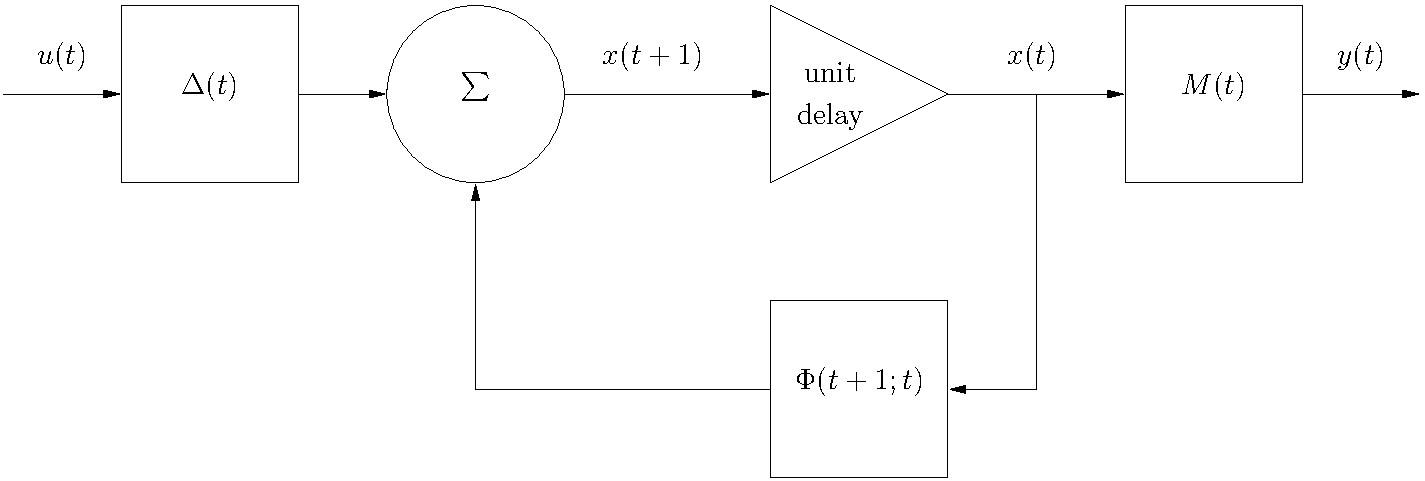
\includegraphics[width=0.5\paperwidth]{fig/fg2.pdf}
\caption{Matrix block diagram of the general linear discrete-dynamic system}
\label{fg2}
\end{figure}
See Fig. 2. One could also express exp Fτ in closed form using
Laplace transform methods [18, 20, 22, 24]. If u(t) satisfies (13)
but the system (12) is nonstationary, we can write analogously
\begin{equation}
\label{eq14}
\left.\begin{aligned}
\mathbf{x}(t+1)&=\boldsymbol{\Phi}(t+1;t)+\boldsymbol{\Delta}(t)\mathbf{u}(t)\\
\mathbf{y}(t)&=\mathbf{M}(t)\mathbf{x}(t)
\end{aligned}\right\}
\qquad t=0,1,\dotsc
\end{equation}
but of course now Φ(t + 1; t), Δ(t) cannot be expressed in general
in closed form. Equations of type (14) are encountered frequently
also in the study of complicated sampled-data systems
[22]. See Fig. 2

Φ(t + 1; t) is the transition matrix of the system (12) or (14).
The notation Φ(t2; t1) (t2, t1 = integers) indicates transition from
time t1 to time t2. Evidently Φ(t; t) = I = unit matrix. If the system
(12) is stationary then Φ(t + 1; t) = Φ(t + 1 – t) = Φ(1) = const.
Note also the product rule: Φ(t; s)Φ(s; r) = Φ(t; r) and the inverse
rule Φ–1(t; s) = Φ(s; t), where t, s, r are integers. In a stationary
system, Φ(t; τ) = exp F(t – τ).

As a result of the preceding discussion, we shall represent random
phenomena by the model
\begin{equation}
\label{eq15}
\mathbf{x}(t+1)=\boldPhi(t+1;t)\mathbf{x}(t)+\mathbf{u}(t)
\end{equation}
where {u(t)} is a vector-valued, independent, gaussian random
process, with zero mean, which is completely described by (in
view of Theorem 5 (C))
\begin{align*}
E\mathbf{u}(t)=0 \text{ for all } t;\\
E\mathbf{u}(t)\mathbf{u'}(s)=0 \text{ if } t \ne s\\
E\mathbf{u}(t)\mathbf{u'}(t)=\mathbf{G}(t).
\end{align*}
Of course (Theorem 5 (A)), x(t) is then also a gaussian random
process with zero mean, but it is no longer independent. In fact, if
we consider (15) in the steady state (assuming it is a stable system),
in other words, if we neglect the initial state x(t0), then
\begin{equation*}
\mathbf{x}(t)=\sum^{t-1}_{r=-\infty}\boldPhi(t;r+1)\mathbf{u}(r).
\end{equation*}
Therefore if t ≥ s we have
\begin{equation*}
E\mathbf{x}(t)\mathbf{x'}(s)=\sum^{s-1}_{r=-\infty}\boldPhi(t;r+1)\mathbf{Q'}(r)\boldsymbol{\Phi'}(s;r+1).
\end{equation*}
Thus if we assume a linear dynamic model and know the
statistical properties of the gaussian random excitation, it is easy
to find the corresponding statistical properties of the gaussian
random process {x(t)}.

In real life, however, the situation is usually reversed. One is
given the covariance matrix Ex(t)x'(s) (or rather, one attempts to
estimate the matrix from limited statistical data) and the problem
is to get (15) and the statistical properties of u(t). This is a subtle
and presently largely unsolved problem in experimentation and
data reduction. As in the vast majority of the engineering
literature on the Wiener problem, we shall find it convenient to
start with the model (15) and regard the problem of obtaining the
model itself as a separate question. To be sure, the two problems
should be optimized jointly if possible; the author is not aware,
however, of any study of the joint optimization problem.

In summary, the following assumptions are made about random
processes:

Physical random phenomena may be thought of as due to
primary random sources exciting dynamic systems. The primary
sources are assumed to be independent gaussian random
processes with zero mean; the dynamic systems will be linear. The
random processes are therefore described by models such as (15).
The question of how the numbers specifying the model are
obtained from experimental data will not be considered.
\section{Solution of the Wiener problem}
\section{The Dual Problem}
\section{Applications}
\section{Conclusions}
\end{document}